
O proxecto desenvolveuse mediante un enfoque \textbf{incremental e iterativo}, empregando un taboleiro \textbf{Kanban} para organizar as tarefas e realizar o seu seguimento. Esta forma de traballo permitiu avanzar por etapas, comprobar os resultados de cada unha e adaptar o desenvolvemento ás necesidades que foron aparecendo.

Optouse por un fluxo continuo de traballo, no que as tarefas se priorizaron segundo a súa importancia para o funcionamento principal do sistema, as dependencias existentes, a dificultade técnica e a proximidade dos fitos establecidos.

\section{Enfoque incremental e iterativo}

O desenvolvemento incremental consiste en construír o sistema mediante etapas sucesivas que amplían progresivamente as súas capacidades. Cada incremento parte dos resultados obtidos nos anteriores e incorpora novas funcionalidades ou melloras.

O carácter iterativo permite revisar e modificar solucións xa desenvolvidas cando aparecen novos datos ou necesidades. Isto foi especialmente importante neste proxecto, xa que a estrutura dos informes, os resultados das tecnoloxías de extracción e os requisitos da aplicación móbil fóronse coñecendo con maior precisión durante o desenvolvemento.

En lugar de desenvolver a aplicación completa desde o principio, o traballo dividiuse en varios pasos. Primeiro estudouse se era posible extraer os datos automaticamente dos documentos, despois desenvolveuse unha API capaz de procesar os informes e, finalmente, creouse a aplicación móbil que consume esa API e permite utilizar os resultados.

Esta forma de traballo evitou desenvolver a aplicación móbil arredor dunha tecnoloxía de extracción que podía non ofrecer resultados suficientemente fiables. Ademais, permitiu comprobar o funcionamento de cada compoñente antes de realizar a integración completa do sistema.


\section{Incrementos do desenvolvemento}
O proxecto dividiuse nos seguintes incrementos:
\begin{enumerate}
    \item \textbf{Estudo da viabilidade e investigación de tecnoloxías de extracción automática:} Analizáronse as características das follas de tratamento, identificáronse os campos que debían ser extraídos e estudáronse  diferentes técnicas de visión artificial, recoñecemento óptico de caracteres e procesamento documental.
    Este incremento permitiu comprender o problema, identificar as principais dificultades e determinar os requisitos básicos da solución.

    \item \textbf{Experimentación e selección da tecnoloxía de extracción:}  Recompiláronse follas de tratamento que se empregaron para probar as distintas tecnoloxías. Avaliáronse alternativas como Tesseract, Google ML Kit, modelos de detección baseados en YOLO e Azure AI Document Intelligence.

     As probas permitiron comparar a calidade da extracción, o esforzo necesario para preparar os datos, a facilidade de integración e as limitacións de cada alternativa. A partir destes resultados seleccionouse a tecnoloxía máis adecuada para continuar o proxecto.

    \item \textbf{Primeira versión da API:} Desenvolveuse unha API sinxela capaz de recibir informes, invocar o servizo de extracción, procesar o resultado e devolver os datos estruturados en formato JSON.

    O obxectivo deste incremento foi obter unha proba de concepto funcional que permitise comprobar a comunicación co servizo de extracción e a transformación dos datos devoltos.

    \item \textbf{Reorganización da API por capas:} Unha vez comprobado o funcionamento da primeira versión, a API reorganizouse para separar os puntos de entrada, a lóxica de negocio, os modelos de datos e as dependencias externas. 

    %TODO: permitiu comprobar os seus compoñentes por separado
    Esta reorganización facilitou o mantemento, a realización de probas e a posible substitución dalgún dos servizos externos no futuro. Neste incremento incorporáronse tamén probas unitarias e probas de integración dos \textit{endpoints}.

    \item \textbf{Primeira versión da aplicación Flutter:} Creouse a estrutura do proxecto Flutter e implementáronse progresivamente a configuración inicial, as modalidades de paciente e supervisor, a persistencia local, a captura de informes, a visualización da pauta, o calendario e a confirmación das tomas.

    As funcionalidades da aplicación dividíronse en tarefas independentes para facilitar a súa implementación e revisión.

    \item \textbf{Integración:}   Neste incremento integrouse a aplicación con Firebase e coa API, conectáronse os diferentes fluxos de navegación e incorporáronse a vinculación entre paciente e supervisor, a sincronización da información e os recordatorios relacionados co tratamento.
    
    A integración realizouse progresivamente, comprobando primeiro os compoñentes por separado e, posteriormente, o funcionamento completo do sistema.

    \item \textbf{Estabilización e probas:} Nesta etapa realizouse a análise estática do código, comprobouse a compilación da aplicación e incorporáronse probas unitarias e de widgets para verificar as funcionalidades principais. Tamén se executaron probas nun dispositivo real, revisáronse a navegación e os principais casos de uso, e corrixíronse os erros detectados.

    \item  \textbf{Documentación e entrega:} O último incremento abrangueu a revisión final da memoria, a elaboración dos diagramas definitivos e a preparación da presentación e dos materiais necesarios para a entrega.

\end{enumerate}

Aínda que o proxecto se organizou nestes incrementos, algunhas actividades desenvolvéronse de forma transversal. A documentación, as probas e determinadas correccións leváronse a cabo durante todo o desenvolvemento, mentres que cada incremento mantivo un obxectivo principal claramente definido.

\section{Taboleiro Kanban}
Kanban é un método de xestión visual que permite representar as tarefas do proxecto segundo o seu estado. Cada tarefa móvese entre distintas columnas a medida que avanza o seu desenvolvemento, o que facilita coñecer o traballo pendente, identificar as actividades que se están realizando e comprobar as que xa foron completadas. No proxecto empregouse un taboleiro de GitHub Projects con catro estados:
\begin{itemize}
    \item \textbf{Para máis adiante:} ideas ou tarefas que non forman parte do traballo inmediato.
    \item \textbf{Por facer:} tarefas xa definidas e priorizadas que aínda non comezaron.
    \item \textbf{En curso:} traballo que se está realizando nese momento.
    \item \textbf{Feito:} tarefas completadas e comprobadas.
\end{itemize}

Unha tarefa non pasa directamente de \textit{Por facer} a \textit{Feito}. Cando comeza o traballo, móvese a \textit{En curso} e permanece nese estado durante a implementación e as comprobacións. Só se move a \textit{Feito} cando se completou o traballo e se realizaron as comprobacións aplicables.

Estableceuse un límite de traballo en curso, ou límite WIP (\textit{Work In Progress}), de \textbf{catro tarefas}. Este límite inclúe tamén tarefas pendentes de revisión, validación ou desbloqueo, polo que non implica que todas se desenvolvan simultaneamente. Escolleuse este valor porque permite manter activas tarefas de distintas áreas do proxecto sen acumular un número excesivo de actividades abertas.

O seu obxectivo é favorecer a finalización das tarefas iniciadas antes de comezar outras novas. Cando se alcanza o límite, priorízase a finalización, integración ou desbloqueo das tarefas existentes.

Na Figura~\ref{fig:taboleiro-kanban} móstrase o estado do taboleiro Kanban nun momento representativo do desenvolvemento, coas tarefas distribuídas segundo o seu estado.

% TODO: Engadir cando o taboleiro teña un estado representativo.
%
% \begin{figure}
%     \centering
%     \includegraphics[width=\linewidth]
%     {imaxes/02-Metodoloxia/taboleiro-kanban.png}
%     \caption{Estado do taboleiro Kanban o XX de XXXXX de 2026.}
%     \label{fig:taboleiro-kanban}
% \end{figure}

\subsection{Estrutura das tarefas}
Cada tarefa representada no taboleiro corresponde a unha issue de GitHub e pode incluír os seguintes elementos:
\begin{multicols}{2}
\begin{itemize}
    \item Unha descrición breve
    \item Unha estimación das horas necesarias
    \item Unha lista de comprobación
    \item Os criterios de aceptación
    \item Unha prioridade
    \item Etiquetas que identifican a área ou tipo de traballo
    \item Un fito que indica a data obxectivo
    \item Referencias ás \textit{pull requests} ou a outras \textit{issues}
\end{itemize}
\end{multicols}

Na Figura~\ref{fig:exemplo-tarefa} preséntase unha das tarefas do proxecto, na que se poden observar algúns destes elementos.

\begin{figure}[h!]
    \centering
    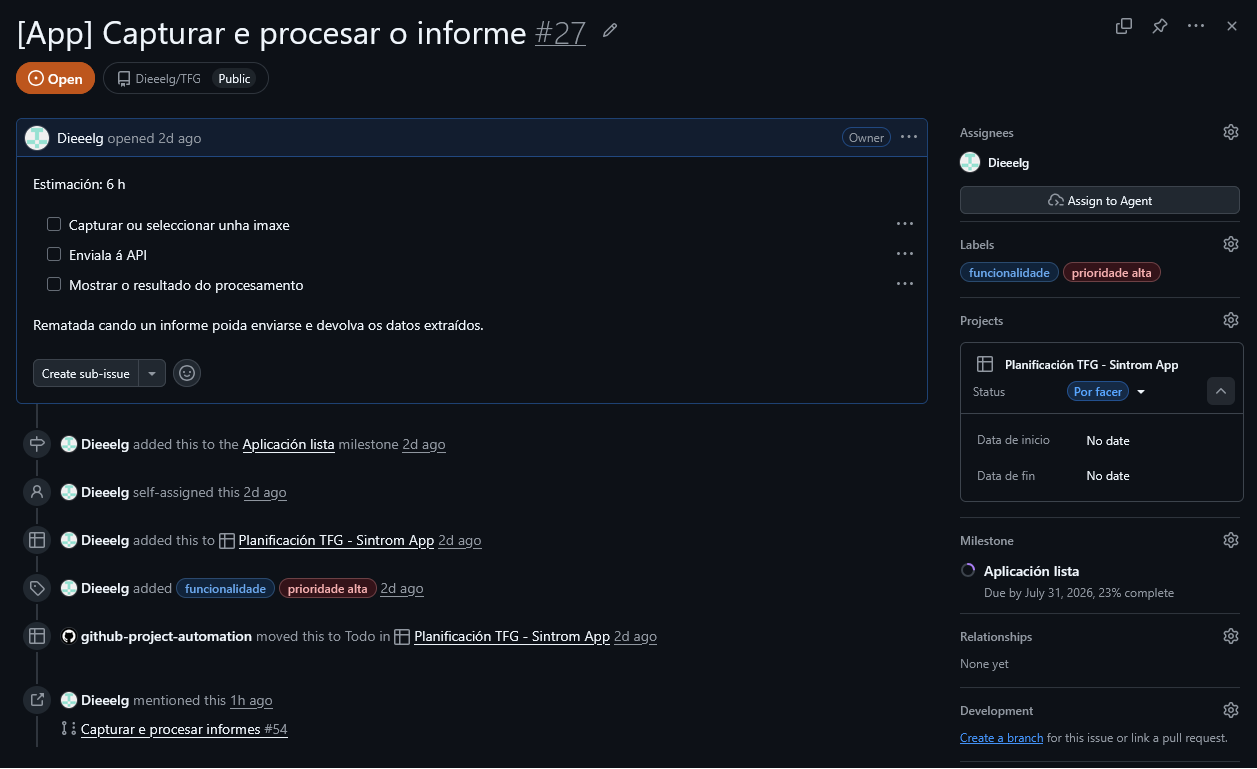
\includegraphics[width=0.8\linewidth]{imaxes/02-Metodoloxía/exemploTarefa.png}
    \caption{Exemplo dunha tarefa do proxecto.}
    \label{fig:exemplo-tarefa}
\end{figure}
\FloatBarrier

As etiquetas permiten clasificar as tarefas segundo o seu tipo, diferenciando entre novas funcionalidades, correccións, melloras, probas, documentación e seguridade. Tamén se empregan etiquetas de prioridade para destacar as tarefas máis urxentes ou aquelas que bloquean o avance do proxecto.

Os fitos permiten agrupar tarefas relacionadas cun mesmo obxectivo ou etapa do desenvolvemento, como completar unha versión funcional da aplicación, realizar as probas, finalizar a memoria ou preparar a entrega do proxecto.


\subsection{Priorización e seguimento}
Para indicar a urxencia das tarefas empregáronse tres etiquetas de prioridade:

\begin{itemize}
    \item \textbf{Prioridade alta}: tarefas que debían realizarse canto antes, especialmente cando bloqueaban o fluxo principal ou outras actividades
    \item \textbf{Prioridade media}: tarefas importantes, pero que non impedían continuar co desenvolvemento
    \item \textbf{Prioridade baixa}: tarefas que podían pospoñerse ata completar as funcionalidades principais
\end{itemize}

As tarefas priorizáronse atendendo principalmente aos seguintes criterios:

\begin{multicols}{2}
\begin{itemize}
    \item a súa importancia para completar o fluxo principal;
    \item as dependencias con outras tarefas;
    \item a dificultade e incerteza técnica;
    \item a proximidade do fito ao que pertencen;
    \item a existencia dun erro que bloquee outras funcionalidades.
\end{itemize}
\end{multicols}

As funcionalidades necesarias para procesar un informe, gardar os datos, consultar a pauta e confirmar unha toma recibiron unha prioridade superior ás melloras visuais. Do mesmo xeito, unha corrección que bloqueaba varias tarefas ten prioridade sobre unha funcionalidade independente que podía incorporarse máis adiante.

O taboleiro revisouse periodicamente e ao finalizar cada incremento. Durante estas revisións comprobouse o estado das tarefas, actualizáronse as prioridades e identificáronse posibles bloqueos.

Cando unha tarefa resultaba demasiado ampla ou combinaba cambios non relacionados, dividíase en tarefas máis pequenas. Isto facilita a estimación, a revisión do código e a comprobación do resultado.

\section{Xestión do desenvolvemento con Git e GitHub}

Git empregouse como sistema de control de versións, mentres que GitHub se utilizou como repositorio remoto e como ferramenta para relacionar a planificación co desenvolvemento do código. As principais ferramentas utilizadas foron:

\begin{itemize}
    \item \textbf{GitHub Issues}, para describir e seguir as tarefas;
    \item \textbf{GitHub Projects}, para representar o taboleiro Kanban;
    \item \textbf{labels}, para clasificar e priorizar o traballo;
    \item \textbf{milestones}, para agrupar tarefas segundo os fitos;
    \item \textbf{ramas}, para separar os cambios;
    \item \textbf{pull requests}, para revisar e integrar o código.
\end{itemize}

Deste xeito, cada tarefa podía seguirse desde a súa creación no taboleiro ata a integración dos cambios correspondentes no código.

\subsection{Estratexia de ramas e commits}
A rama \textit{master} reservouse para as versións estables, mentres que a rama \textit{develop} se empregou como rama de integración, na que se incorporaron progresivamente os cambios comprobados. Para desenvolver cada tarefa creouse unha rama específica. Utilizáronse os seguintes prefixos:

\begin{itemize}
    \item \textit{feature/}, para novas funcionalidades;
    \item \textit{fix/}, para correccións ou cambios que solucionan un problema.
    \item \textit{release/}, para preparar unha versión antes de publicala
\end{itemize}

Os nomes das ramas describen brevemente o seu obxectivo, como \textit{feature/gardar-datos}, \textit{feature/calendario} ou \textit{fix/configuracion-local}.

Procurouse que cada commit agrupase un cambio concreto e coherente. As mensaxes incluíron descricións breves acompañadas de prefixos como \textit{feat}, \textit{fix}, \textit{refactor} ou \textit{chore}, segundo a natureza da modificación realizada.

%TODO REVISAR
%Esta estratexia non constitúe unha aplicación completa de GitFlow, xa que non se empregaron todas as ramas e procedementos definidos por ese modelo. Trátase dun fluxo simplificado inspirado nel, suficiente para separar o desenvolvemento, as correccións e as versións estables dun proxecto individual.

A estratexia empregada está baseada en GitFlow, xa que diferencia entre unha rama estable, unha rama de integración e ramas específicas para funcionalidades, correccións e preparación de versións. As ramas \texttt{hotfix/} quedarían reservadas para posibles correccións urxentes sobre unha versión xa publicada.

\subsection{Pull requests e integración}

Os cambios realizados en cada rama de traballo integráronse mediante unha \textit{pull request}. A súa descrición incluíu un resumo dos cambios, as comprobacións realizadas e as \textit{issues} relacionadas.

Cando unha funcionalidade aínda necesitaba revisión ou probas, a \textit{pull request} mantíñase como borrador. Este estado permitía facer visible o traballo sen presentalo como preparado para a integración.

Antes de integrar os cambios realizáronse as comprobacións aplicables segundo o compoñente modificado:

\begin{itemize}
    \item verificar que os cambios se correspondían co obxectivo da tarefa;
    \item comprobar que non se incluían credenciais, configuracións locais ou datos sensibles;
    \item evitar a incorporación de ficheiros xerados innecesarios;
    \item comprobar que non existían conflitos coa rama de integración;
    \item revisar a descrición da \textit{pull request} e as referencias ás \textit{issues};
    \item confirmar o cumprimento dos criterios de aceptación.
\end{itemize}

No caso da aplicación Flutter, executouse a análise estática mediante o comando \textit{flutter analyze}, comprobouse a compilación da aplicación e realizáronse as probas unitarias, de widgets e funcionais aplicables.

No caso da API, executáronse as probas unitarias e de integración relacionadas cos compoñentes modificados e comprobouse o comportamento dos \textit{endpoints} afectados.

Unha vez superadas as comprobacións, os cambios integrábanse na rama \textit{develop}. A continuación, pechábase a \textit{issue} correspondente e a tarefa movíase á columna \textit{Feito} do taboleiro.

Na Figura~\ref{fig:exemplo-pr} móstrase unha das \textit{pull requests} empregadas para documentar e integrar os cambios.

\begin{figure}[h!]
    \centering
    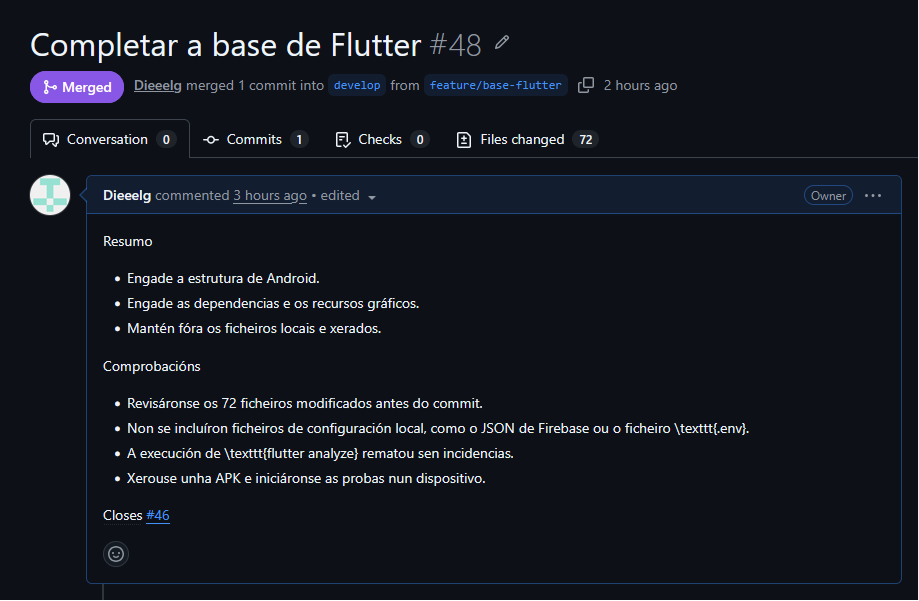
\includegraphics[width=0.8\linewidth]
    {imaxes/02-Metodoloxía/PR.png}
    \caption{Exemplo dunha \textit{pull request} do proxecto.}
    \label{fig:exemplo-pr}
\end{figure}
\FloatBarrier

\subsection{Fluxo de traballo dunha tarefa}

O fluxo habitual seguido para desenvolver unha tarefa foi o seguinte:

\begin{enumerate}
    \item seleccionar unha \textit{issue} priorizada no taboleiro
    \item revisar o seu obxectivo, as dependencias e os criterios de aceptación
    \item mover a tarefa á columna \textit{En curso}
    \item crear unha rama específica a partir da rama de integración
    \item implementar os cambios mediante commits
    \item publicar a rama no repositorio remoto
    \item crear unha \textit{pull request}, inicialmente como borrador
    \item realizar as comprobacións técnicas e funcionais
    \item integrar os cambios na rama \textit{develop}
    \item pechar a \textit{issue} e mover a tarefa á columna \textit{Feito}
\end{enumerate}

Este fluxo permitiu seguir cada tarefa desde a súa planificación ata a integración dos cambios e garantiu que non se considerase rematada antes de realizar as comprobacións correspondentes.

\section{Xustificación da metodoloxía}

A combinación dun desenvolvemento incremental e iterativo cun taboleiro Kanban resultou axeitada para as características e necesidades do proxecto. Durante as primeiras etapas existía unha elevada incerteza sobre a viabilidade da extracción automática dos datos e sobre a tecnoloxía máis axeitada para realizala. Por este motivo, resultaba difícil establecer desde o inicio unha planificación pechada ou estimar con precisión a duración das tarefas de investigación e experimentación.

O enfoque incremental permitiu avanzar por etapas e reducir progresivamente esta incerteza. Primeiro estudouse a viabilidade da extracción automática, despois seleccionouse unha tecnoloxía e desenvolveuse unha primeira versión funcional da API e, finalmente, construíuse a aplicación móbil. Cada incremento proporcionou un resultado comprobable que serviu como base para continuar co desenvolvemento.

O carácter iterativo permitiu revisar solucións xa desenvolvidas cando se obtiveron novos resultados. As decisións relacionadas coa extracción dos datos, a organización da API e o funcionamento da aplicación fóronse modificando e refinando a medida que se coñecían mellor a estrutura dos informes e as necesidades do sistema.

Non se aplicou Scrum de maneira estrita porque a organización do traballo en sprints de duración fixa non se considerou a opción máis axeitada para unhas tarefas cunha duración e uns resultados difíciles de prever. En cambio, Kanban permitiu manter un fluxo continuo, modificar as prioridades segundo os avances realizados e incorporar novas tarefas cando se detectaban necesidades ou problemas.

O taboleiro proporcionou unha representación visual do estado do proxecto, diferenciando as tarefas pendentes, as que se atopaban en desenvolvemento e as que xa foran comprobadas. O límite de traballo en curso favoreceu a finalización das tarefas iniciadas antes de abrir novas liñas de traballo e permitiu identificar aquelas que permanecían pendentes de revisión ou validación.

GitHub completou esta organización ao relacionar a planificación coa implementación. Mediante as \textit{issues}, as ramas, os commits e as \textit{pull requests}, cada cambio podía asociarse coa tarefa que o motivaba e coas comprobacións realizadas antes da súa integración.

Como principal limitación, ao tratarse dun proxecto individual non se contou cunha revisión técnica continua realizada por outra persoa. Para reducir este risco empregáronse listas de comprobación, ferramentas de análise estática, probas automatizadas, comprobacións de compilación e probas manuais dos principais fluxos da aplicación.
